\chapter{MÔ PHỎNG VÀ THỰC NGHIỆM}
     \section{Mô phỏng}
          \subsection{Thông số mô phỏng robot}
               \hspace*{0.6cm}Thực hiện mô phỏng chuyển động của Robot sau khi tìm được hàm truyền của động cơ bằng cách nhúng hàm truyền động cơ,
               bộ điều khiển tốc độ, sai số cảm biến cùng với bộ điều khiển vị trí bám line với các thông số như sau:
               \begin{table}[h]
                    \centering
                    \begin{tabular}{|l|c|}
                    \hline
                    \multicolumn{2}{|c|}{\textbf{Thông số hình học}} \\
                    \hline
                    Bán kính bánh xe, $r$ & 68 mm \\
                    \hline
                    Khoảng cách từ tâm dây cảm biến đến trục bánh dẫn động, $a$ & 72 mm \\
                    \hline
                    Khoảng cách dọc trục giữa tâm 2 bánh xe, $b$ & 220 mm \\
                    \hline
                    \multicolumn{2}{|c|}{\textbf{Thời gian}} \\
                    \hline
                    Thời gian lấy mẫu bộ điều khiển động cơ, $t_{\text{s}}$ & 0.01 s \\
                    \hline
                    Thời gian lấy mẫu bộ điều khiển bám line, $t_{\text{đk}}$ & 0.05 s \\
                    \hline
                    \multicolumn{2}{|c|}{\textbf{Bộ điều khiển PID}} \\
                    \hline
                    Vị trí bám line & $K_P = 0.078$; $K_D = 0.015$ \\
                    \hline
                    Động cơ phải & $K_P = 1.0852$; $K_I = 13.6563$ \\
                    \hline
                    Động cơ trái & $K_P = 1.0673$; $K_I = 13.948$ \\
                    \hline
                    \multicolumn{2}{|c|}{\textbf{Thông số động học}} \\
                    \hline
                    Vận tốc của robot, $v$ & 500 mm/s \\
                    \hline
                    Vận tốc của robot lúc vào cua, $v_{\text{r}}$ & 300 mm/s \\
                    \hline
                    Góc lệch ban đầu, $p$ & $\pi$ \\
                    \hline
                    \end{tabular}
                    \label{tab:robot_specifications}
                    \caption{Thông số đầu vào mô phỏng chuyển động của robot}
               \end{table}
          \subsection{Thực hiện mô phỏng}
               \hspace*{0.6cm}Mô phỏng bằng phần mềm MATLAB, bước đầu tiên là tạo sa bàn với các kích thước như trong đầu bài
               \begin{figure}[H]
                    \centering
                    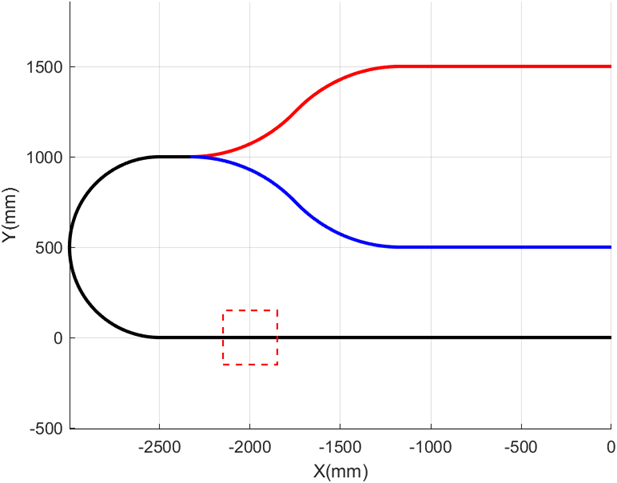
\includegraphics[width=0.8\textwidth]{pictures/chapter8/saban.png}
                    \caption{Hình ảnh sa bàn}
                    \label{saban}
               \end{figure}
               \hspace*{0.6cm}Trong đó đường line màu đỏ và màu xanh lần lượt thể hiện nhánh rẽ khi xe nhận được khối hàng màu đỏ và xanh. Tại khu vực nhận hàng, mô phỏng quá trình đặt tải màu lên xe bằng 1 cửa sổ trong đó người dùng chọn màu sắc của khối hàng.
               \begin{figure}[H]
                    \centering
                    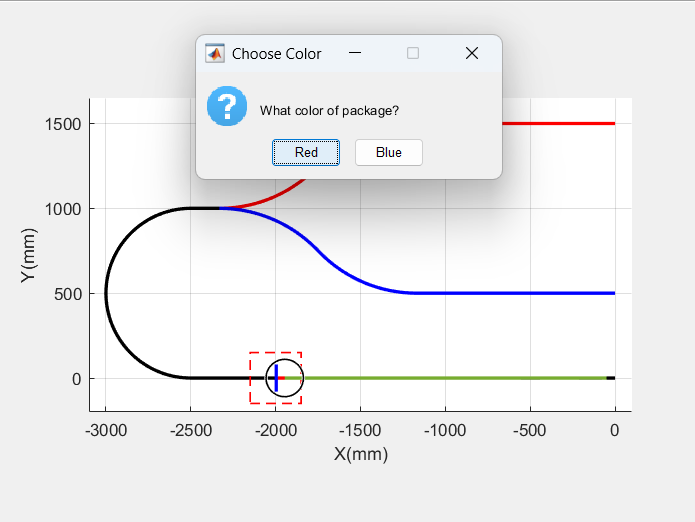
\includegraphics[width=0.8\textwidth]{pictures/chapter8/stop_for_package.png}
                    \caption{Chọn màu sắc gói hàng}
                    \label{choose_color}
               \end{figure}
               \hspace*{0.6cm}Tùy thuộc vào màu sắc khối hàng mà sau khi gặp ngã rẽ, xe sẽ rẽ lên trên hoặc xuống dưới.
               \begin{figure}[H]
                    \centering
                    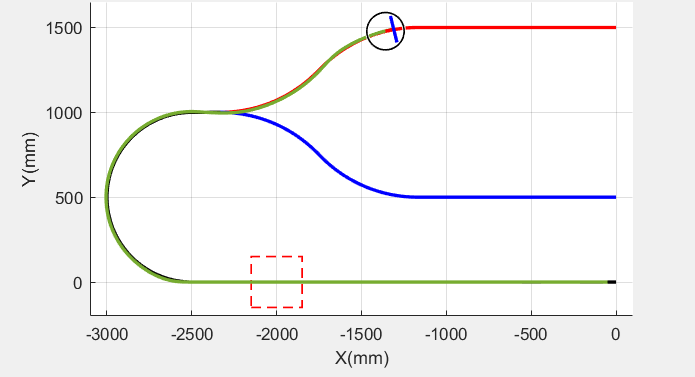
\includegraphics[width=0.9\textwidth]{pictures/chapter8/running.png}
                    \caption{Hình ảnh xe chạy mô phỏng}
                    \label{running}
               \end{figure}     

          \subsection{Kết quả mô phỏng}
          Thực hiện mô phỏng xe chạy với vận tốc 0.3 m/s.
          \begin{itemize}
               \item \textbf{Khối hàng đỏ}
                    \begin{figure}[H]
                         \centering
                         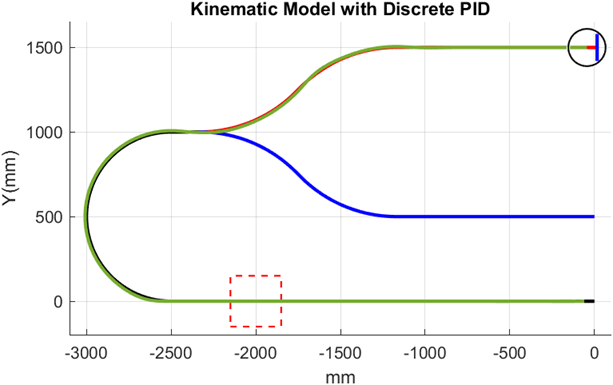
\includegraphics[width=1\textwidth]{pictures/chapter8/trajec_red.png}
                         \caption{Quỹ đạo đi khi nhận khối hàng đỏ}
                         \label{tra_red}
                    \end{figure}
                    \begin{figure}[H]
                         \centering
                         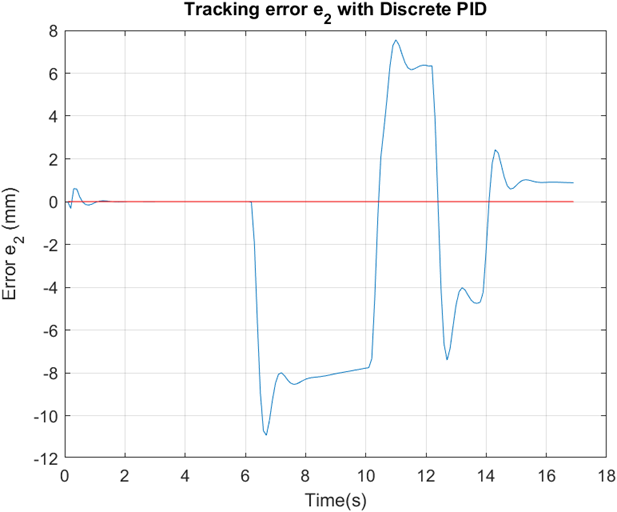
\includegraphics[width=0.9\textwidth]{pictures/chapter8/err_red.png}
                         \caption{Lỗi quỹ đạo e2 khi nhận khối hàng đỏ}
                         \label{err_red}
                    \end{figure}
               \textbf{*Nhận xét:}
               \begin{itemize}
                    \item Sai số lệch lớn nhất giữa tâm cảm biến và tâm đường line là khoảng 11 mm.
                    \item Sai số bám line trên đoạn thẳng (< 6s) rất nhỏ, tuy nhiên khi xe bắt đầu vào cua thì sai số tăng dần đến đạt lớn nhất là -11 mm (thể hiện xe lệch qua phía trái đường line). 
               \end{itemize}

               \item \textbf{Khối hàng xanh}
          \end{itemize}
               
          \subsection{Khối hàng xanh}
               \begin{figure}[H]
                    \centering
                    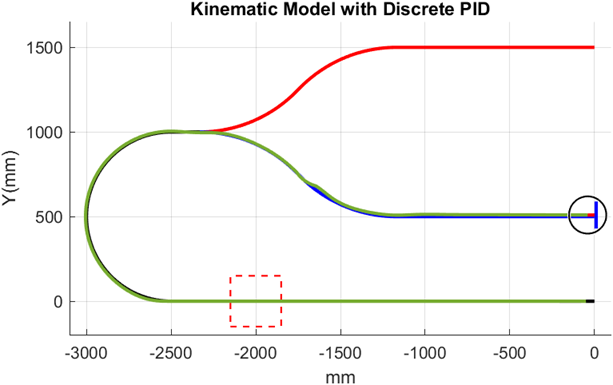
\includegraphics[width=0.8\textwidth]{pictures/chapter8/trajec_blue.png}
                    \caption{Quỹ đạo đi khi nhận khối hàng xanh}
                    \label{tra_blue}
               \end{figure}
               \begin{figure}[H]
                    \centering
                    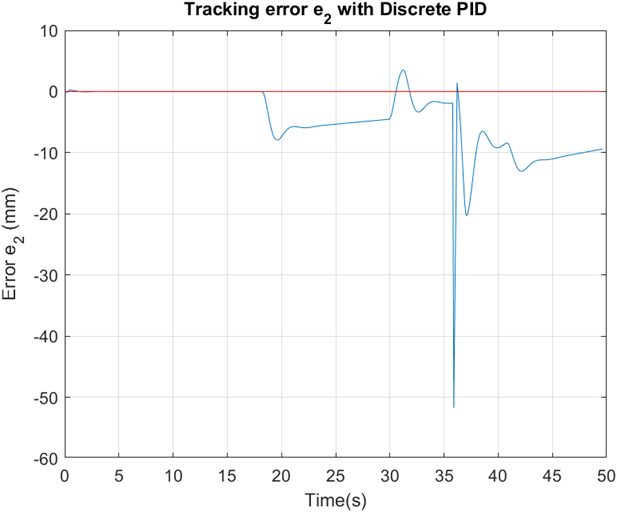
\includegraphics[width=0.9\textwidth]{pictures/chapter8/err_blue.png}
                    \caption{Lỗi quỹ đạo e2 khi nhận khối hàng xanh}
                    \label{err_blue}
               \end{figure}
               \textbf{*Nhận xét:}
               \begin{itemize}
                    \item Sai lệch trung bình giữa tâm cảm biến và tâm đường line trên toàn bộ đoạn đường là khoảng 4 mm.
                    \item Sai số bám line trên đoạn thẳng (< 6s) rất nhỏ, tuy nhiên khi xe bắt đầu vào cua thì sai số tăng dần, có 1 vị trí xe bị lệch ra khỏi line khoảng 50 mm, sau đó bám vào lại line và di chuyển tới cuối đường. 
               \end{itemize}
     \section{Thực nghiệm}
          \subsection{Kết quả thực nghiệm}
               \begin{figure}[H]
                    \centering
                    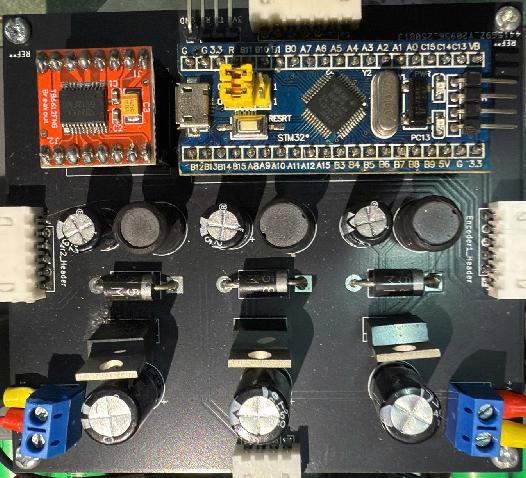
\includegraphics[width=0.7\textwidth]{pictures/chapter8/PCB.png}
                    \caption{Mạch PCB điều khiển}
                    \label{PCB}
               \end{figure}
               \begin{figure}[H]
                    \centering
                    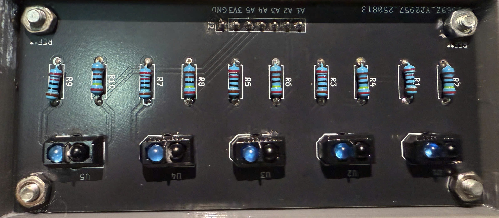
\includegraphics[width=0.7\textwidth]{pictures/chapter8/sensor.png}
                    \caption{Mạch cảm biến dò line}
                    \label{line_sensor}
               \end{figure}
               \begin{figure}[H]
                    \centering
                    \begin{minipage}{0.42\textwidth}
                         \centering
                         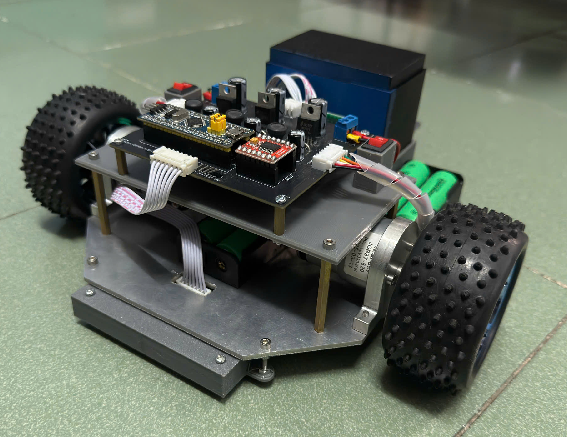
\includegraphics[width=\linewidth]{pictures/chapter8/xe_full1.png}
                    \end{minipage}\hfill
                    \begin{minipage}{0.42\textwidth}
                         \centering
                         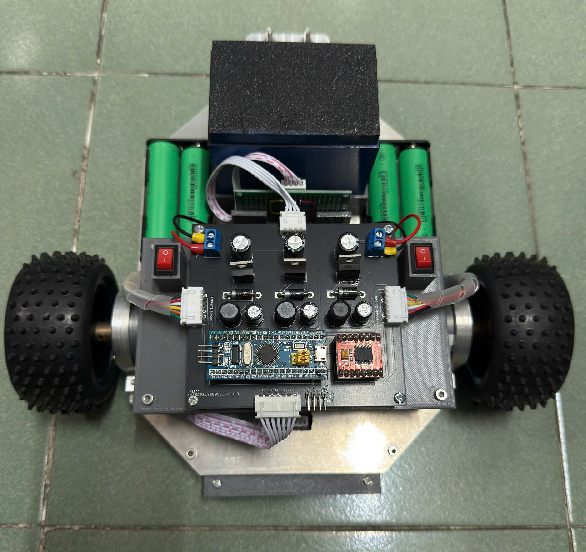
\includegraphics[width=\linewidth]{pictures/chapter8/xe_full2.png}
                    \end{minipage}
                    \caption{Robot dò line sau khi đã lắp hoàn chỉnh}
                    \label{xe_full}
               \end{figure}
               \begin{figure}[H]
                    \centering
                    \begin{minipage}{0.5\textwidth}
                         \centering
                         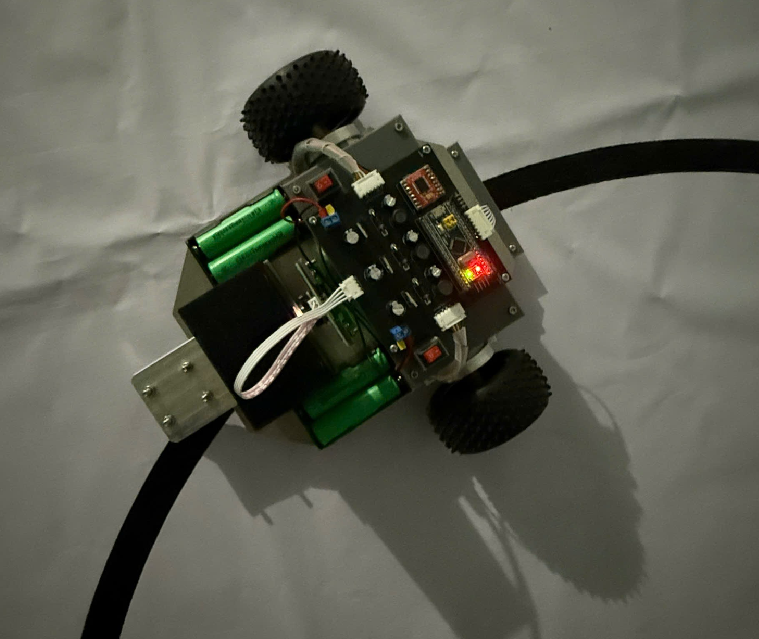
\includegraphics[width=\linewidth]{pictures/chapter8/turn.png}
                         \caption{Xe rẽ vào đoạn cua R500}
                         \label{fig:chapter8:1.2 - 1}
                    \end{minipage}\hfill
                    \begin{minipage}{0.42\textwidth}
                         \centering
                         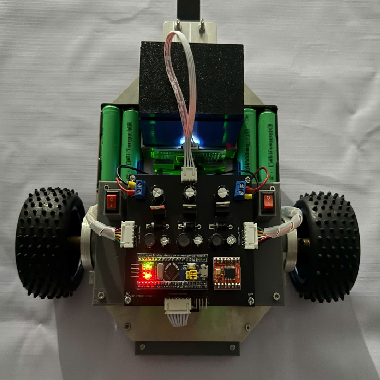
\includegraphics[width=\linewidth]{pictures/chapter8/end.png}
                         \caption{Xe dừng cuối line}
                         \label{fig:chapter8:1.2 - 4}
                    \end{minipage}
                    \vspace{0.5cm}

                    \begin{minipage}{0.5\textwidth}
                         \centering
                         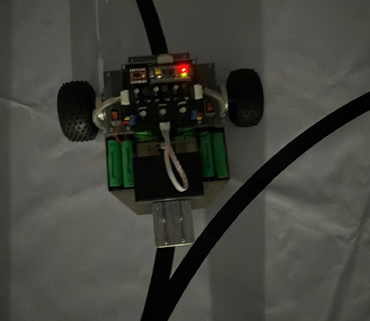
\includegraphics[width=\linewidth]{pictures/chapter8/turn_left.png}
                         \caption{Xe rẽ trái khi nhận hàng màu đỏ}
                         \label{fig:chapter8:1.2 - 2}
                    \end{minipage}\hfill
                    \begin{minipage}{0.42\textwidth}
                         \centering
                         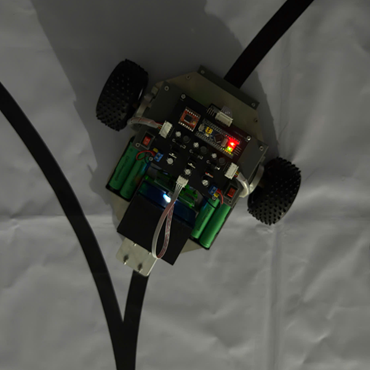
\includegraphics[width=\linewidth]{pictures/chapter8/turn_right.png}
                         \caption{Xe rẽ phải khi nhận hàng màu xanh}
                         \label{fig:chapter8:1.2 - 3}
                    \end{minipage}
               \end{figure}
          \hspace*{0.6cm}Robot được chạy thử nghiệm trên sa bàn in với kích thước giống kích thước của đầu bài. Khu vực tải hàng được đại diện bằng 1 đường line đen dài 50mm, rộng 26mm và cách vị trí xuất phát đầu line 2000mm. Robot được thử nghiệm chạy với các tốc độ khác nhau $0.3 \,\mathrm{m/s}, \,  0.5 \,\mathrm{m/s}, \, 0.8 \,\mathrm{m/s}$.\\
               \hspace*{0.6cm}\textbf{Nhận xét:}
               \begin{itemize}
                    \item Với vận tốc $v = 0.3 \,\mathrm{m/s}$, xe di chuyển chậm, khá ổn định. Thời gian hoàn thành khoảng 28 đến 30 giây.
                    \item Với vận tốc $v = 0.5 \,\mathrm{m/s}$, xe di chuyển trên đường thẳng ổn định. Thời gian hoàn thành khoảng 18 đến 22 giây.
                    \item Với vận tốc $v = 0.8 \,\mathrm{m/s}$, xe di chuyển nhanh, đoạn line thẳng xe đi rất ổn định nếu lúc đầu đặt tâm dãy cảm biến của xe ở chính giữa line, nếu đặt hơi lệch có thể dẫn đến xe hơi lắc trong quá trình chạy. Thời gian hoàn thành khoảng 10 đến 15 giây.
               \end{itemize}
          \subsection{Đánh giá}
               \begin{itemize}
                    \item Với nhiệm vụ bám line, xe thực hiện bám line khá tốt cả trên đoạn line thẳng và đoạn vào cua.
                    \item Tại khu vực nhận hàng, xe dừng để chờ nhận tải và chờ nhận đúng màu sắc trong đề bài (xanh hoặc đỏ) mới tiếp tục hoàn thành quãng đường còn lại.
                    \item Về bộ điều khiển PID vận tốc động cơ 2 bánh, kết quả các hệ số của bộ điều khiển tìm được nhờ công cụ Tuning của MATLAB khá sát với các hệ số khi triển khai code thực tế vì đều sử dụng bộ điều khiển PID dạng rời rạc, chứng tỏ bước lấy mẫu động cơ, tìm hàm truyền và sử dụng MATLAB để tìm các hệ số cho bộ điều khiển là quan trọng, giúp cho việc triển khai thực tế dễ dàng hơn. 
               \end{itemize}
          \subsection{Kết luận}
               \hspace*{0.6cm}Qua đề tài thiết kế xe dò line phân phối hàng hóa theo màu sắc, nhóm đã thực hiện được các mục tiêu sau:
               \begin{itemize}
                    \item Tìm hiểu tổng quan về các mô hình AGVs nói chung và xe dò line nói riêng.
                    \item Biết được cách thực hiện dự án theo hướng thiết kế hệ thống cơ điện tử.
                    \item Học được các bước thiết kế hệ cơ khí, lắp ráp các bộ phận của robot.
                    \item Học được cách tính toán, chọn các linh kiện điện tử và thiết kế mạch in PCB.
                    \item Hoàn thành bộ hồ sơ thiết kế thỏa mãn các yêu cầu của đồ án trong thời gian quy định.
               \end{itemize}